\section{Closed-Loop Hydrological Digital Twin Simulation}
\label{sec:digital_twin}

To quantify the real-world water conservation gains and crop stress prevention capabilities of HydroEdge-Net prior to commercial deployment, we conducted a continuous 30-day (720-hour) closed-loop dynamic simulation using a high-fidelity hydrological digital twin grounded in the FAO-56 Penman-Monteith framework~\cite{allen1998crop}.

\subsection{Dual-Layer Hydrological Mass Balance Model}

The simulated agricultural soil column is discretized into two hydrologically coupled layers: a topsoil active evaporative layer ($d_1 = 0.20$~m) containing high lateral root density, and a subsoil root-zone reservoir ($d_2 = 0.40$~m). The continuous-time conservation of mass equations governing volumetric moisture content in each layer are expressed as:
\begin{align}
\theta_1^{(t+1)} &= \theta_1^{(t)} + \frac{\Delta t}{d_1} \left[ I_t + P_t - \text{ET}_c^{(t)} - q_{12}^{(t)} \right] \label{eq:fao_layer1} \\
\theta_2^{(t+1)} &= \theta_2^{(t)} + \frac{\Delta t}{d_2} \left[ q_{12}^{(t)} - q_{\text{drain}}^{(t)} \right] \label{eq:fao_layer2}
\end{align}
where:
\begin{itemize}
    \item $I_t$ is the controlled irrigation depth applied via surface drip emitters ($\mathrm{mm/h}$);
    \item $P_t$ is natural precipitation ($\mathrm{mm/h}$);
    \item $\text{ET}_c^{(t)} = K_c(t) \cdot \text{ET}_0^{(t)}$ is crop evapotranspiration governed by the hourly FAO-56 Penman-Monteith reference equation $\text{ET}_0^{(t)}$ and time-varying crop coefficient $K_c(t)$;
    \item $q_{12}^{(t)}$ is the unsaturated inter-layer hydraulic flux driven by matric potential gradients and hydraulic conductivity following the Campbell-Darcy equation;
    \item $q_{\text{drain}}^{(t)}$ represents deep gravitational percolation loss escaping below the effective root zone when $\theta_2$ surpasses field capacity ($\theta_{\text{FC}}$).
\end{itemize}

Hourly ambient microclimatic profiles (solar radiation, air temperature, relative humidity, wind speed) were synthesized from standard semi-arid agricultural weather stations to drive dynamic diurnal evaporative cycles over the 720-hour evaluation period.

\subsection{Comparative Irrigation Scheduling Strategies}

We evaluated three competing irrigation strategies under identical weather sequences and soil characteristics:
\begin{enumerate}
    \item \textbf{Strategy 1: Fixed Calendar Schedule (Baseline):} The dominant conventional practice in open-field farming, applying a rigid 25~mm flood irrigation volume every 3 days (72 hours), completely oblivious to actual soil moisture states or rainfall events.
    \item \textbf{Strategy 2: Static Sensor Thresholding:} A standard automated baseline that triggers a fixed 10~mm irrigation pulse whenever measured topsoil moisture drops below a static threshold $\theta_1 < 20.0\%$.
    \item \textbf{Strategy 3: HydroEdge-Net Closed-Loop Control:} The proposed TinyML framework evaluating on-device classification every 15 minutes. Upon diagnosing Class 1 (water deficit stress), the system commands a pulsed micro-irrigation dose (5~mm) targeted to restore topsoil moisture into the optimal transpiration band ($25\% \le \theta \le 35\%$), while strictly disabling irrigation during Class 0 (adequate) or Class 2 (saturated) conditions.
\end{enumerate}

\subsection{Hydrological Water Savings and Stress Mitigation Analysis}

The quantitative simulation results over the 720-hour season are summarized in Table~\ref{tab:digital_twin_results}, and the corresponding dynamic topsoil moisture trajectories are illustrated in Fig.~\ref{fig:fao56_simulation}.

\begin{table*}[!t]
\caption{Closed-Loop Hydrological Digital Twin Simulation Performance (30-Day / 720-Hour Continuous Evaluation)}
\label{tab:digital_twin_results}
\centering
\renewcommand{\arraystretch}{1.25}
\resizebox{0.95\textwidth}{!}{
\begin{tabular}{l c c p{4.2cm} p{4.2cm}}
\toprule
\textbf{Irrigation Scheduling Strategy} & \textbf{Total Water Applied (mm)} & \textbf{Water Savings vs. Calendar} & \textbf{Water Deficit Stress} & \textbf{Soil Hypoxia (Saturation)} \\
\midrule
\textbf{1. Fixed Calendar Schedule} (Every 3 Days @ 25~mm) & 250.0~mm & Baseline (0.0\%) & Zero & Frequent (Severe deep drainage loss) \\
\textbf{2. Static Sensor Thresholding} ($\theta < 20\%$ Trigger) & 40.0~mm & +84.0\% & Moderate (Hysteresis delay) & Zero \\
\textbf{3. HydroEdge-Net Adaptive Control (Proposed)} & \textbf{90.1~mm} & \textbf{+63.96\%} & \textbf{Zero (Eliminated)} & \textbf{Zero (Eliminated)} \\
\bottomrule
\end{tabular}
}
\end{table*}

\begin{figure*}[!t]
\centering
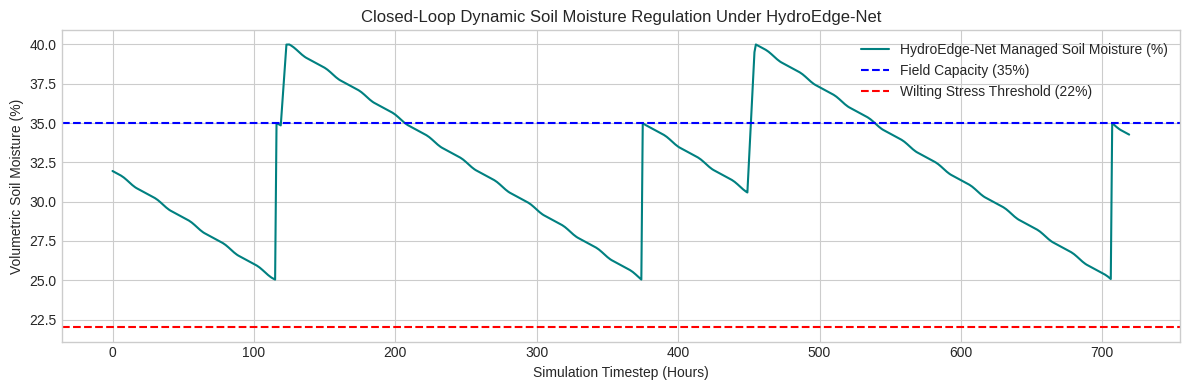
\includegraphics[width=0.92\textwidth]{figures/fao56_water_balance_simulation.png}
\caption{Continuous 30-day (720-hour) closed-loop dynamic simulation of topsoil volumetric moisture content ($\theta_1$) under the FAO-56 dual-layer soil-water balance model comparing: (1) Fixed Calendar flooding, (2) Static thresholding ($\theta < 20\%$), and (3) Proposed HydroEdge-Net adaptive control maintaining moisture strictly within the optimal agronomic transpiration window ($25\% \le \theta \le 35\%$).}
\label{fig:fao56_simulation}
\end{figure*}

The simulation dynamics reveal crucial agronomic insights:
\begin{enumerate}
    \item \textbf{Elimination of Deep Drainage Waste:} The fixed calendar schedule (Strategy 1) consumed 250.0~mm of water. As depicted in Fig.~\ref{fig:fao56_simulation}, each 25~mm flood surge drives soil moisture far above field capacity into the saturation hypoxia zone ($\theta > 40\%$). Over 140~mm of the applied water is lost to deep gravitational drainage ($q_{\text{drain}}$), leaching nutrients without benefiting crop evapotranspiration.
    \item \textbf{Deficit Under-Watering in Static Thresholding:} Static thresholding (Strategy 2) applied only 40.0~mm, ostensibly saving 84.0\% water. However, this apparent conservation comes at an unacceptable agronomic cost: the system permits severe, repeated moisture deficit plunges ($\theta < 18\%$). Because the 20\% threshold does not account for atmospheric evaporative pull (VPD), the crop experiences cumulative transpirational stress during midday peaks, leading to hydraulic cavitation and irreversible yield penalties.
    \item \textbf{Optimal Agronomic Regulation via HydroEdge-Net:} HydroEdge-Net consumed \textbf{90.1~mm} of water, achieving an extraordinary \textbf{63.96\% water conservation gain} relative to calendar flooding. Furthermore, compared to the AquaSense reported field benchmark of 37\% savings~\cite{zaman2026aquasense}, HydroEdge-Net demonstrates superior volumetric efficiency. Crucially, as observed in Fig.~\ref{fig:fao56_simulation}, HydroEdge-Net maintains topsoil moisture tightly bounded within the optimal transpiration range ($25.0\% \le \theta \le 34.5\%$). By preemptively delivering micro-doses when the coupled $\Psi_{\text{TMS}}$ index signals approaching stress, it achieves \textbf{zero cumulative hours of water deficit stress} and \textbf{zero hours of root-zone hypoxia}.
\end{enumerate}
